Construct thereafter the Hamiltonian matrix for a system with no broken pairs and total spin $S = 0$ for the case of the four lowest single-particle levels indicated in the Fig.~\ref{fig:schematic}.
Our system consists of four particles only.
Our single-particle space consists of only the four lowest levels $p= 1, 2, 3, 4$.
You need to set up all possible Slater determinants.
Find all eigenvalues by diagonalizing the Hamiltonian matrix.
Vary your results for values of $g \in [-1, 1]$.
We refer to this as the exact calculation.
Comment the behavior of the ground state as function of $g$.

\subsection{}
Due to the requirement of no broken pairs, total spin $S = 0$, and the fact that we have four particles, the number of possible Slater determinants is quite limited.
We choose our ansatz $\ket{\Phi_0}$ to be the Slater determinant with all four particles below the Fermi level of $p = 2$.
The possible Slater determinants are shown in Fig.~\ref{fig:SDs}.

\begin{figure}[htbp]
    \centering
    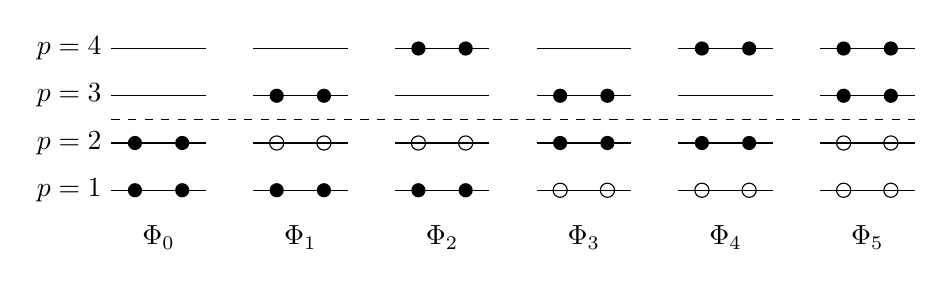
\begin{tikzpicture}[scale=0.6]
        % Draw lines
        \foreach \x in {0,3,6,9,12,15} {
            \foreach \y in {1,2,3,4} {
                \draw (\x, \y) -- (\x+2, \y);
            }
        }
        % Draw additional dashed lines
        \draw[dashed] (0, 2.5) -- (17, 2.5);

        % Labels on the left
        \foreach \y/\label in {1/$p=1$, 2/$p=2$, 3/$p=3$, 4/$p=4$} {
            \node[left] at (0, \y) {\label};
        }

        % Groundstate
        \foreach \x/\y in {0.5/1, 0.5/2, 1.5/1, 1.5/2} {
            \fill (\x, \y) circle (0.15);
        }
        \node at (1, 0) {$\ket{\Phi_0}$};

        % Phi_1
        \foreach \x in {3.5, 4.5} {
            \foreach \y in {1, 3} {
                \fill (\x, \y) circle (0.15);
            }
            \draw (\x, 2) circle (0.15);
        }
        \node at (4, 0) {$\ket{\Phi_1}$};

        % Phi_2
        \foreach \x in {6.5, 7.5} {
            \foreach \y in {1, 4} {
                \fill (\x, \y) circle (0.15);
            }
            \draw (\x, 2) circle (0.15);
        }
        \node at (7, 0) {$\ket{\Phi_2}$};

        % Phi_3
        \foreach \x in {9.5, 10.5} {
            \foreach \y in {2, 3} {
                \fill (\x, \y) circle (0.15);
            }
            \foreach \y in {1} {
                \draw (\x, \y) circle (0.15);
            }
        }
        \node at (10, 0) {$\ket{\Phi_3}$};

        % Phi_4
        \foreach \x in {12.5, 13.5} {
            \foreach \y in {2, 4} {
                \fill (\x, \y) circle (0.15);
            }
            \foreach \y in {1} {
                \draw (\x, \y) circle (0.15);
            }
        }
        \node at (13, 0) {$\ket{\Phi_4}$};

        % Phi_5
        \foreach \x in {15.5, 16.5} {
            \foreach \y in {3, 4} {
                \fill (\x, \y) circle (0.15);
            }
            \foreach \y in {1, 2} {
                \draw (\x, \y) circle (0.15);
            }
        }
        \node at (16, 0) {$\ket{\Phi_5}$};

    \end{tikzpicture}
    \caption{
        Schematic representation of the six possible Slater determinants for a system with four particles, under the constraint of no broken pairs, total spin $S = 0$, considering only the four lowest levels $p = 1, 2, 3, 4$.\label{fig:SDs}
    }
\end{figure}

Setting up the Slater determinants in second quantization, we set the ground state to be
\begin{equation*}
    \ket{\Phi_0} = a_{1+}^\dagger a_{1-}^\dagger a_{2+}^\dagger a_{2-}^\dagger \ket{0},
\end{equation*}
or equivalently with the pair creation operators
\begin{equation*}
    \ket{\Phi_0} = \hat{P}_1^+ \hat{P}_2^+ \ket{0}.
\end{equation*}
The other Slater determinants are then
\begin{align*}
    \ket{\Phi_1} &= \hat{P}_1^+ \hat{P}_3^+ \ket{0}, &
    \ket{\Phi_2} &= \hat{P}_1^+ \hat{P}_4^+ \ket{0}, \\
    \ket{\Phi_3} &= \hat{P}_2^+ \hat{P}_3^+ \ket{0}, &
    \ket{\Phi_4} &= \hat{P}_2^+ \hat{P}_4^+ \ket{0}, \\
    \ket{\Phi_5} &= \hat{P}_3^+ \hat{P}_4^+ \ket{0}.
\end{align*}
Equivalently, we can write these relative to the ground state as
\begin{align*}
    \ket{\Phi_1} &= \hat{P}_3^+ \hat{P}_2^- \ket{\Phi_0}, \\
    \ket{\Phi_2} &= \hat{P}_4^+ \hat{P}_2^- \ket{\Phi_0}, &
    \ket{\Phi_3} &= \hat{P}_3^+ \hat{P}_1^- \ket{\Phi_0}, \\
    \ket{\Phi_4} &= \hat{P}_4^+ \hat{P}_1^- \ket{\Phi_0}, &
    \ket{\Phi_5} &= \hat{P}_4^+ \hat{P}_3^+ \hat{P}_1^- \hat{P}_2^- \ket{\Phi_0}.
\end{align*}
Note that as the pair creation and annihilation operators commute, the order of the operators in the Slater determinants is not important.

We define an arbitrary four-particle state $\ket{\Phi}_{\alpha, \beta}$, with $\alpha < \beta$, as
\begin{equation*}
    \ket{\Phi}_{\alpha, \beta} = \hat{P}_\alpha^+ \hat{P}_\beta^+ \ket{0}
\end{equation*}
in order to simplify the computation for the Hamiltonian matrix.
For $\langle \Phi_{\alpha, \beta} | \hat{H}_0 | \Phi_{\gamma, \delta} \rangle$, we only need to consider the terms where $(\alpha, \beta) = (\gamma, \delta)$, as the other terms vanish due to the orthogonality of the Slater determinants.
\begin{align*}
    \langle \Phi_{\alpha, \beta} | \hat{H}_0 | \Phi_{\alpha, \beta} \rangle
    &= \langle \Phi_{\alpha, \beta} | \sum_{p\sigma} (p - 1) a_{p\sigma}^\dagger a_{p\sigma} | \Phi_{\alpha, \beta} \rangle \\
    &= \sum_{p\sigma} (p - 1) \langle \Phi_{\alpha, \beta} | a_{p\sigma}^\dagger a_{p\sigma} | \Phi_{\alpha, \beta} \rangle \\
    &= \sum_{\substack{p=\alpha,\beta\\ \sigma=\pm}} (p - 1) \\
    &= 2(\alpha - 1) + 2(\beta - 1) \\
    &= 2(\alpha + \beta - 2).
\end{align*}

% For $\langle \Phi_{\alpha, \beta} | \hat{V} | \Phi_{\gamma, \delta} \rangle$, we first consider the terms along the diagonal where $(\alpha, \beta) = (\gamma, \delta)$.
% \begin{align*}
%     \langle \Phi_{\alpha, \beta} | \hat{V} | \Phi_{\alpha, \beta} \rangle
%     &= -\frac{1}{2} g \sum_{pq} \langle \Phi_{\alpha, \beta} | \hat{P}_p^+ \hat{P}_q^- | \Phi_{\alpha, \beta} \rangle \\
%     &= -\frac{1}{2} g \sum_{pq} \langle 0 | \hat{P}_\beta^- \hat{P}_\alpha^- \hat{P}_p^+ \hat{P}_q^- \hat{P}_\alpha^+ \hat{P}_\beta^+| 0 \rangle
% \end{align*}
% The possible contractions are then
% \begin{align*}
%     \wick{
%         \left\langle 0 \left\vert
%         \c2 {\hat{P}_\beta^-}
%         \c1 {\hat{P}_\alpha^-}
%         \c1 {\hat{P}_p^+}
%         \c1 {\hat{P}_q^-}
%         \c1 {\hat{P}_\alpha^+}
%         \c2 {\hat{P}_\beta^+}
%         \right\vert 0 \right\rangle
%     } &= \delta_{\alpha p} \delta_{\alpha q}, \\
%     \wick{
%         \left\langle 0 \left\vert
%         \c1 {\hat{P}_\beta^-}
%         \c2 {\hat{P}_\alpha^-}
%         \c1 {\hat{P}_p^+}
%         \c1 {\hat{P}_q^-}
%         \c2 {\hat{P}_\alpha^+}
%         \c1 {\hat{P}_\beta^+}
%         \right\vert 0 \right\rangle
%     } &= \delta_{\beta p} \delta_{\beta q}.
% \end{align*}

Next, we consider $\langle \Phi_{\alpha, \beta} | \hat{V} | \Phi_{\gamma, \delta} \rangle$.
\begin{align*}
    \langle \Phi_{\alpha, \beta} | \hat{V} | \Phi_{\gamma, \delta} \rangle
    &= -\frac{1}{2} g \sum_{pq} \langle \Phi_{\alpha, \beta} | \hat{P}_p^+ \hat{P}_q^- | \Phi_{\gamma, \delta} \rangle \\
    &= -\frac{1}{2} g \sum_{pq} \langle 0 | \hat{P}_\beta^- \hat{P}_\alpha^- \hat{P}_p^+ \hat{P}_q^- \hat{P}_\gamma^+ \hat{P}_\delta^+| 0 \rangle
\end{align*}
The possible contractions are then
\begin{align*}
    (1) \quad \wick[offset=1.2em,sep=0.3em]{
        \left\langle 0 \left\vert
        \c2 {\hat{P}_\beta^-}
        \c1 {\hat{P}_\alpha^-}
        \c1 {\hat{P}_p^+}
        \c1 {\hat{P}_q^-}
        \c1 {\hat{P}_\gamma^+}
        \c2 {\hat{P}_\delta^+}
        \right\vert 0 \right\rangle
    } &= \delta_{\beta \delta} \delta_{\alpha p} \delta_{q \gamma} \\[0.5em]
    (2) \quad \wick[offset=1.2em,sep=0.3em]{
        \left\langle 0 \left\vert
        \c2 {\hat{P}_\beta^-}
        \c1 {\hat{P}_\alpha^-}
        \c1 {\hat{P}_p^+}
        \c1 {\hat{P}_q^-}
        \c2 {\hat{P}_\gamma^+}
        \c1 {\hat{P}_\delta^+}
        \right\vert 0 \right\rangle
    } &= -\delta_{\beta \gamma} \delta_{\alpha p} \delta_{q \delta} \\[0.5em]
    (3) \quad \wick[offset=1.2em,sep=0.3em]{
        \left\langle 0 \left\vert
        \c1 {\hat{P}_\beta^-}
        \c2 {\hat{P}_\alpha^-}
        \c1 {\hat{P}_p^+}
        \c1 {\hat{P}_q^-}
        \c2 {\hat{P}_\gamma^+}
        \c1 {\hat{P}_\delta^+}
        \right\vert 0 \right\rangle
    } &= \delta_{\beta p} \delta_{\alpha \gamma} \delta_{q \delta} \\[0.5em]
    (4) \quad \wick[offset=1.2em,sep=0.3em]{
        \left\langle 0 \left\vert
        \c1 {\hat{P}_\beta^-}
        \c2 {\hat{P}_\alpha^-}
        \c1 {\hat{P}_p^+}
        \c1 {\hat{P}_q^-}
        \c1 {\hat{P}_\gamma^+}
        \c2 {\hat{P}_\delta^+}
        \right\vert 0 \right\rangle
    } &= -\delta_{\beta p} \delta_{\alpha \delta} \delta_{q \gamma}
\end{align*}
From this, we can then calculate the matrix elements of the Hamiltonian matrix based on the number of matched pairs.
When two pairs match, i.e.~along the diagonal, we get contributions from $(1)$ and $(3)$.
When one pair matches and the other differs, we get contributions from \textit{either} $(2)$ or $(4)$.
When no pairs match, the matrix element is zero.

From this, we can set up the Hamiltonian matrix for the system, ordered as $\ket{\Phi_0}, \ket{\Phi_1}, \ldots, \ket{\Phi_5}$.
\begin{align*}
    H &= H_0 + V \\
    &=
    \begin{bmatrix}
        2 & 0 & 0 & 0 & 0 & 0 \\
        0 & 4 & 0 & 0 & 0 & 0 \\
        0 & 0 & 6 & 0 & 0 & 0 \\
        0 & 0 & 0 & 6 & 0 & 0 \\
        0 & 0 & 0 & 0 & 8 & 0 \\
        0 & 0 & 0 & 0 & 0 & 10
    \end{bmatrix}
    - \frac{g}{2}
    \begin{bmatrix}
        2 & 1 & 1 & 1 & 1 & 0 \\
        1 & 2 & 1 & 1 & 0 & 1 \\
        1 & 1 & 2 & 0 & 1 & 1 \\
        1 & 1 & 0 & 2 & 1 & 1 \\
        1 & 0 & 1 & 1 & 2 & 1 \\
        0 & 1 & 1 & 1 & 1 & 2
    \end{bmatrix} \\
    &=
    \begin{bmatrix}
        2 - g & - \frac{g}{2} & - \frac{g}{2} & - \frac{g}{2} & - \frac{g}{2} & 0 \\
        - \frac{g}{2} & 4 - g & - \frac{g}{2} & - \frac{g}{2} & 0 & - \frac{g}{2} \\
        - \frac{g}{2} & - \frac{g}{2} & 6 - g & 0 & - \frac{g}{2} & - \frac{g}{2} \\
        - \frac{g}{2} & - \frac{g}{2} & 0 & 6 - g & - \frac{g}{2} & - \frac{g}{2} \\
        - \frac{g}{2} & 0 & - \frac{g}{2} & - \frac{g}{2} & 8 - g & - \frac{g}{2} \\
        0 & - \frac{g}{2} & - \frac{g}{2} & - \frac{g}{2} & - \frac{g}{2} & 10 - g
    \end{bmatrix}
\end{align*}
We diagonalize this matrix for varying values of $g \in [-1, 1]$ with NumPy, computed in the script \verb|b.py|.
Plotted as a function of $g$, the eigenvalues are shown in Fig.~\ref{fig:b_eigenvalues}, while the ground state energy is shown in Fig.~\ref{fig:b_groundstate}.
% TODO: Comment on the behavior of the ground state as a function of $g$.

\begin{figure}[htbp]
    \centering
    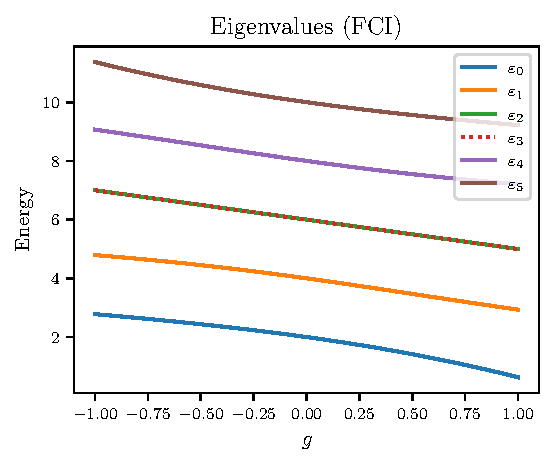
\includegraphics{figures/b_eigenvalues_energy.pdf}
    \caption{
        Eigenvalues of the Hamiltonian matrix for the four-particle system with no broken pairs and total spin $S = 0$, as a function of the pairing strength $g$.\label{fig:b_eigenvalues}
    }
\end{figure}

\begin{figure}[htbp]
    \centering
    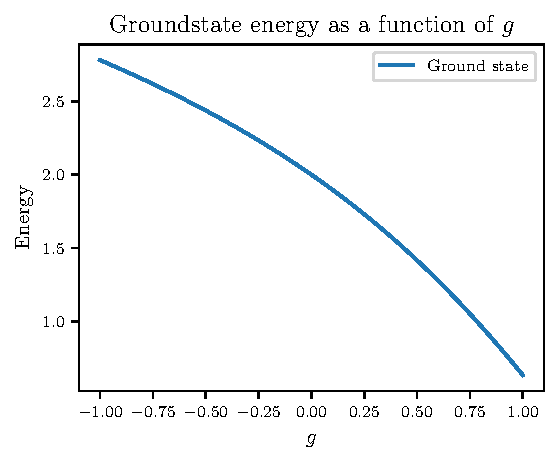
\includegraphics{figures/b_ground_state_energy.pdf}
    \caption{
        Ground state energy of the Hamiltonian matrix for the four-particle system with no broken pairs and total spin $S = 0$, as a function of the pairing strength $g$.\label{fig:b_groundstate}
    }
\end{figure}

